\usepackage[utf8]{inputenc}
\usepackage[T1]{fontenc}
\usepackage{mathptmx}
\usepackage[scaled=.90]{helvet}
\usepackage{courier}
\usepackage{caption}
\captionsetup{labelformat=empty,labelsep=none}
\usepackage{verbatim}
\usepackage{hyperref}
\usepackage{listings}
\lstset{language=Perl,basicstyle=\normalsize,tabsize=3,showstringspaces=false}

\title{Interchange 6 - Open Source Shop Machine}
\author[racke]{Stefan Hornburg (Racke)\\ \texttt{racke@linuxia.de}}
\date{16. Deutscher Perl-Workshop, Hannover, 28. März 2013}

\begin{document}
\maketitle{}

\begin{frame}
  \titlepage
\end{frame}

\tableofcontents

\section{Übersicht}

Eine Auswahl von Online-Shopsysteme, die in Deutschland häufig eingesetzt
werden. Alle sind in PHP programmiert. Magento wurde von eBay aufgekauft
und hat eine komplizierte Datenbankstruktur.
 
\begin{frame}{Shopsoftware}
  \begin{itemize}
  \item Magento
  \item Shopware
  \item Oxid
  \end{itemize}
\end{frame}

\begin{frame}{PHP Cauldron}
  \begin{center}
    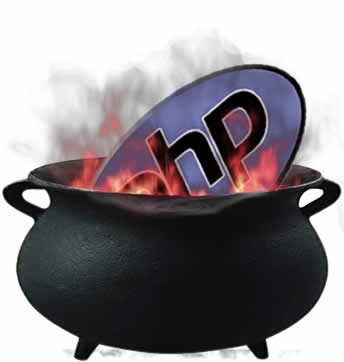
\includegraphics[width=\textwidth,height=0.8\textheight,keepaspectratio]{images/cauldron.jpg}
  \end{center}
\end{frame}

\section{Komponenten}
\begin{frame}{Komponenten ``Manager''}
  \begin{itemize}
  \item DBIx::Class
  \item Moo
  \item Dancer
  \item Template::Flute
  \end{itemize}
\end{frame}

\section{Status Quo}
\begin{frame}{Status Quo}
 \item Interchange6::Schema
  \item Dancer::Plugin::Interchange6
\end{frame}

\begin{frame}{Infos}
Slides:
\url{http://www.linuxia.de/talks/pws2014/interchange6-de-beamer.pdf}
\end{frame}

\end{document}

%%% Local Variables: 
%%% mode: latex
%%% TeX-master: t
%%% End: 
